
\section{Modely}
\label{sec:modely}
Všetky modely pre trénovanie sú implementované v scripte \textit{models.py}.
Existuje jedna hlavná trieda \textit{class Model}, ktorá obsahuje všetky základné atributy potrebné pre modely, ako napr.
    meno modelu, vstupný rozmer dát, zvolený algoritmus trénovania a slovník, ktorý obsahuje indexi a názvy označení obrázkov.

Každý model následne dedí z tejto hlavnej triedy a implementuje v sebe dve funkcie \textit{build}, ktorá zabezpečuje vytvorenie modelu a
    funkciu \textit{train}, ktorá sa volá pri spustení trénovania daného modelu.

\begin{figure}[H]
    \centering
    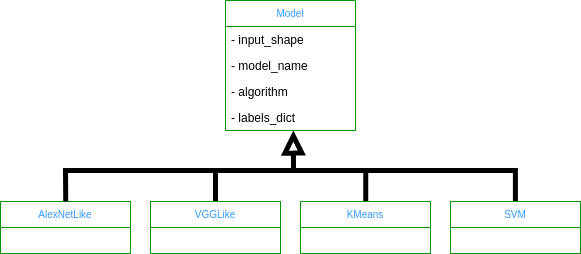
\includegraphics[width=1\textwidth]{inheritance}
    \caption{Hierarchia dedenia tried modelov.}
    \label{pic:inheritance}
\end{figure}

Konvolučné neurónové siete sú implementované pomocou triedy \textit{Sequencia} z knižnice Keras.
Pre klasifikátor K-Nearest-Neighbor je použitá trieda \textit{KNeighborsClassifier} a trieda \textit{SVC} pre klasifikátor SVM z knižnice scikit-learn.

%Pre klasifikátor K-Nearest-Neighbor je použitá trieda \textit{KNeighborsClassifier} s počtom 1 a 5 najbližších susedov, a trieda \textit{SVC} pre klasifikátor SVM
%    so základnými nastavenia trénovania z knižnice scikit-learn.

\subsection{Ukladanie a načítanie modelu}
\label{subsec:ukladaniemodelu}
Pre ukladanie natrénovaných modelov je implemtovaná funkcia \textit{save\_model()} v triede \textit{DataSaver} v scripte \textit{loader.py}.
Pri ukladaní modelu sa ukladá model v binárnej forme, ukladá sa konfiguračný súbor \textit{settings.json}, ktorý obsahuje informácie ako veľkosť
    vstupných dát, použité funkcie na predspracovanie dát, meno modelu, typ algoritmu učenia, zoznam indexov označenia dát a dalšie informácie
    špecifické pre daný typ modelu.
Uložením konvolučnej neurónovej siete sa ukladá graf priebehu trénovanie.

Naopak pre načítanie modelov je implementovaná funkcia \textit{load\_model\_data()} v triede \textit{DataLoader} v scripte \textit{loader.py},
    ktorá načíta binárnu podobu modelu a všetky informácie z konfiguračného súboru \textit{settings.json}.

\subsection{Trénovanie modelov}
\label{sec:trenovanie}
Pre trénovanie modelov sú v rámci implementácie použité všetky triedy, ktoré boli podrobne opísané vyššie.
Proces trénovania prebieha v niekoľkých krokoch.
\begin{enumerate}
    \item Načítanie vstupných dát.
    \item Predspracovanie načítaných dát.
    \item Rozdelenie predspracovaných dát do viacerých skupín.
    
    \begin{figure}[H]
        \centering
        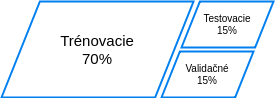
\includegraphics[width=0.45\textwidth]{rozdelenie_dat_3}
        \quad
        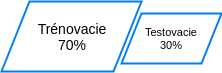
\includegraphics[width=0.45\textwidth]{rozdelenie_dat_2}
        \caption{Rozdelenie dát do skupín, na 3 skupiny pre CNN a na 2 skupiny pre K-means a SVM klasifikátor.}
        \label{pic:datagroups}
    \end{figure}

    %dát na trénovacie, validačné a testovanie v pomere 70\%:15\%:15\% pre konvolučné neurónové siete.
    %A v pomere 70\%:30\% na trénovacie a testovanie pre K-means a SVM klasifikátor.

    \item Vytvorenie modelu.
    \item Spustenie trénovania vytvoreného modelu.
    \item Uloženie natrénovaného modelu a konfiguračného súboru.
    \item Testovanie presnosti modelu pomocou testovacích dát.
\end{enumerate}

Pre uľahčenie trénovania je implementovaný script \textit{train.py}, ktorý požaduje niekoľko argumentov na vstupe.
Zoznam vstupných argumentov a ich význam, argumenty v hranatých zátvorkách sú voliteľné:
\begin{enumerate}
    \item[$\bullet$] \textbf{--model} cesta k priečinku do ktorého bude natrénovaný model uložený.
    \item[$\bullet$] \textbf{--dataset} cesta k priečinku z ktorého budú načítane vstupné dáta.
    \item[$\bullet$] \textbf{--alg} voľba modelu, ktorý bude trénovaný, tento argument má niekoľko možností.
    Možnosť ``cnnc'' pre trénovanie konvolučnej neurónovej siete určenej na klasifikáciu zbrane,
    ``cnna'' pre trénovanie konvolučnej neurónovej siete pre určenie náklonu zbrane a
    ``svm'' alebo ``kmeans'' pre trénovanie SVM alebo K-nearest-neighbor klasifikátora na určenie typu zbrane.
    \item[$\bullet$] \textbf{[--ep]} pri konvolučných neurónových sieťach určuje počet epóch, pri jeho nezadaní je použitá
    základná hodnota 45.
    \item[$\bullet$] \textbf{[--bs]} určuje veľkosť batch-size pri trénovaní konvolučných neurónových sietí, jeho
    základná hodnota je 16.
    \item[$\bullet$] \textbf{[--rt]} je argument, ktorý je potrebné zadať pri trénovani sietí na určenie náklonu zbrane,
    jeho hodnota určuje uhol náklonu, na ktorý sa sieť bude učiť, možné hodnoty argumentu sú: ``yaw'', ``roll'', ``pitch''.
\end{enumerate}

\subsection{Presnosť modelov}
\label{subsec:presnostmodelov}
Pre celkové hodnotenie presnosti modelov bola implementovaná funkcia \textit{evaluate\_model} v scripte \textit{evaluation.py}.
Hodnotí presnosť modelov podľa metrík spomenutých v \ref{subsec:hodnoteniepresnosti}.

V prípade určenia typu zbrane sa používa kontigenčná matica a hodnota celkovej úspešnosti modela.
Táto metrika je použitá aj počas trénovania CNN na predbežné určenie presnosti a taktiež pri koncovom testovaní modelov.

Avšak v prípade CNN, ktoré určujú náklon zbrane je potrebné túto metriku trošku pozmeniť.
Ako je opísané v \ref{subsec:odchylkachyby}, v scripte \textit{base.py} je implementovaná funkcia \textit{angle\_error}, ktorá ráta priemerny rozdiel medzi
    skutočnymi a predpovedanými uhlami siete.
Táto funkcia je použitá ako metrika počas trénovania CNN a pri koncovom testovaní presnosti siete.
Následne po určení či je predikcia správna alebo nie, pomocou prahovej hodnoty, sa použije výpočet úspešnosti z hodnôt v chybovej matici.
